%----------------------------------------------------------------------------
\chapter{Measurements and scaling}
\label{cha:measurements}
%----------------------------------------------------------------------------

After each implementation iteration I measured the performance of the created framework, and continued the development using the results of these measurements. As we previously saw the heart of the framework is the SAT solver, which is also the most time consuming part of the system. So the best way to improve the speed of the execution is to improve the underlying Alloy program.

I created a testing tool to measure the execution of the different Alloy programs. This testing tool can be configured to compare the execution of different Alloy programs, with different execution strategy. The execution strategy can mean different SAT solvers, and other solver configurations as well.

Execution of each testing configuration was measured 10 times and the results in the following section always refer to average metrics. The tests has been running on the configuration that can be seen in Table~\ref{tab:hardwarespecification}.

\begin{table}[htb]
\begin{center}
\begin{tabular}{p{2cm}p{12cm}}
\toprule
	\multicolumn{2}{c}{\textbf{Hardware specification}}\\\midrule
	\textbf{CPU} & 2.7GHz dual-core Intel Core i5 processor with 3MB shared L3 cache\\
	\textbf{RAM} & 8GB 1866MHz LPDDR3 RAM\\
	\textbf{Storage} & 128GB PCIe-based flash storage\\
\bottomrule
\end{tabular}
\end{center}
\caption{\label{tab:hardwarespecification} Measurement architecture}
\end{table}

\section{Alloy settings}
\label{sec:alloysettings}

During the first measurement I experimented with the available solvers supported by Alloy and their solver specific configurations. Alloy Analyzer supports huge variety of SAT solvers and they have a decent number of tuning possibility.

I was able to integrate seven different SAT solvers into the system, namely CryptoMiniSat \cite{cryptominisat}, Glucose \cite{glucose}, MiniSat \cite{minisat}, MiniSat with core extraction, Sat4j \cite{sat4j}, Lingeling \cite{lingeling} and its parallel version Plingeling. The another dimension of the measurement was the SAT solver configuration. Settings of two configuration was not obvious, that's why I chose to measure these parameters.

The first investigated option was Skolem-depth that controls the maximum depth of alternating universal and existential quantifier when generating a Skolem function. Minimum value is 0, which means it will only generate Skolem constants, and will not generate Skolem functions, maximum value is 4, where Skolem functions are generated in depth of 4.

\begin{figure}[htp]
\centering
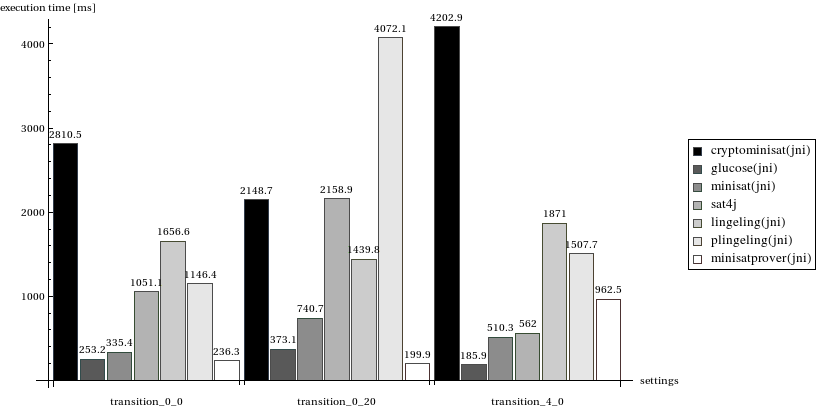
\includegraphics[scale=0.55]{figures/measurements_alloy_settings}
\caption{Adjusting Alloy settings}
\label{fig:measurements_alloy_settings}
\end{figure}

Second option to inspect was symmetry breaking. The official documentation suggests that  if a formula is unsatisfiable, then in general, the higher this value, the faster the solver will finish. On the other hand, if the formula is satisfiable, then the value should be set to a lower value. Minimum of symmetry breaking is 0, maximum is 20.

Figure~\ref{fig:measurements_alloy_settings} shows the results of the measurement. On the x-axis are the solver configurations in the form: \mbox{<\textit{test selection criterion}>\_<\textit{Skolem-depth}>\_<\textit{symmetry breaking}>}. On y-axis is the execution time, and the different colours represent different SAT solver implementations.

The result was similar with state and transition coverage criteria as well, therefore here only the transition coverage version is demonstrated. Measurement with Skolem-depth of 4 and symmetry breaking of 20 is not presented, because this configuration could not satisfy the given problem in acceptable period of time.

The fastest solver became the award winning Glucose SAT solver. Only the MiniSat solvers could approach the performance of Glucose, the other solvers seemed to be significantly slower. That's why Glucose became the default solver of the testing framework.

Symmetry breaking with a value of 0 was also a clear choice, since the documentation suggest that the programs solves satisfiable problem with a lower value more easily. 

Changing the Skolem-depth did not impact the speed very much, only a small amount of difference could be measured. Glucose was faster with an option 0, which was also the default value, so I did not change that.

\begin{figure}[htp]
\centering
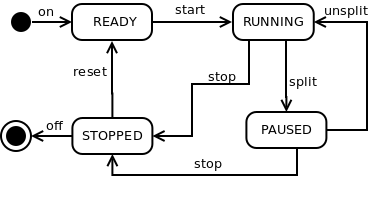
\includegraphics[scale=0.5]{figures/measurements_stopwatch}
\caption{Stopwatch FSM for testing}
\label{fig:measurements_stopwatch}
\end{figure}

Later, as I improved the test generation algorithms, I checked whether these options still held. The framework was still the fastest with this configuration, which was also not surprising, because Alloy documentation recommends this configuration regardless of the model complexity.

As an input for the first two measurements I used an example FSM that represents a simplified stopwatch behaviour (Figure~\ref{fig:measurements_stopwatch}). 

% section alloysettings (end)

\section{Optimisations}
\label{sec:optimalisations}

After the first measurements the performance of the test generation seemed to be adequate to work with, but as I increased the complexity of the problems to solve, so increased the execution time of the test generation. 

The input model, as I mentioned earlier was the stopwatch FSM (Figure~\ref{fig:measurements_stopwatch}) that is ideal for testing purposes, because on the test suite of this stopwatch full state and transition coverage can be achieved and therefore both of the implemented algorithms can be tested.

In the first development iteration, the test generation algorithm could not generate test cases for this FSM within a tolerable time. This was a huge problem, as it could jeopardise the success of using constraint solving methods for test generation. After examining the test generation process and the results with Alloy Analyzer, I identified the main issues.

The first problem was that the model was overconstrained and that's why the SAT solver generated to much variables, while parsing the given constraints. The other problem was that, the solver generated different objects in a scenario for the same purpose, that's why state space increased exponentially.

Solution for these problems is the same: the Alloy model needs to be simplified. This has been done in two steps,  Figure~\ref{fig:measurements_optimalizations} shows the effects of the optimisations. After deleting the unneeded constraints from the model, each SAT solver could solve the stopwatch problem. The execution time at this time displayed with the label "Original" on Figure~\ref{fig:measurements_optimalizations}. Later I modified the model to reuse the previously generated model objects to reduce the state explosion.

\begin{figure}[htp]
\centering
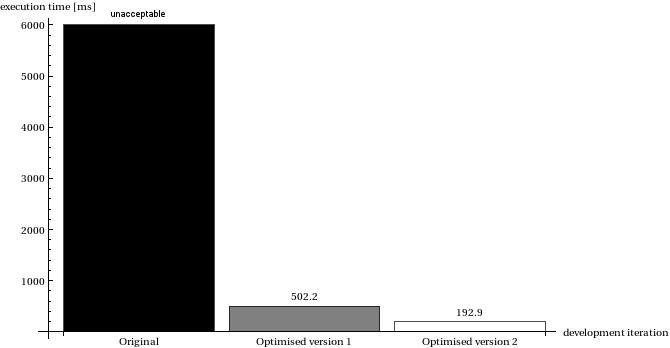
\includegraphics[scale=0.55]{figures/measurements_optimalizations}
\caption{Optimisations results}
\label{fig:measurements_optimalizations}
\end{figure}

The speed of the execution increased radically during these optimisations. In the first step, the increase can not be calculated, as the speed was unacceptable in the first version. Considering the speed of the chosen SAT solver, Glucose, the execution became twice as faster, than previously.

% section optimalizations (end)

\section{Scalability}
\label{sec:scalability}

In the first measurement I investigated the scalability of the created testing framework. I assumed that the test generation algorithm does not scale equally regarding the number of states or transitions generated during the test case generation. That's why I measured the performance considering these two options.

First applicable PLCspecif models have to be generated in different sizes, that are input models of the framework. Then the test generation process can be started using these models where the execution speed is measurable.

Creating a random PLCspecif model, that can represent a SUT, where different test selection criteria can be satisfied is not an easy task, as it involves complex graph theory algorithms to generate such a graph representation. Main parts of the process are the following:

\begin{enumerate}
	\item At first a graph model of the SUT have to be generated. Process of the graph generation is demonstrated in Algorithm~1.
	
\begin{algorithm}
\label{alg:sutmodelgeneration}
\SetAlgoLined
\KwData{$n, t$ such that $t$ is the type of the generation scope for a $G(V,E)$ graph,\\
and $n=$
\begin{cases}
|V|, $ if $ t = $ state$\\
|E|, $ if $ t = $ transition$
\end{cases}
}
\KwResult{$G(V,E)$ graph representation of the SUT}
$s \leftarrow 0$\;
\While{$s \neq n$}{
$in\_degree\_sequence \leftarrow [0] + \mathrm{random\ sequence} + [1]$\;
$out\_degree\_sequence \leftarrow [1] + \mathrm{random\ sequence} + [0]$\;
\While{$|in| \neq |out|$}{
$out\_degree\_sequence \leftarrow [1] + \mathrm{random\ sequence} + [0]$\;
}
$G(V,E) \leftarrow$ random directed pseudograph, using the degree sequences\;
\If{$\exists e \in E: e=(v,v): v \in V$} {
$E\leftarrow E \setminus e$\;
}
$s =$\begin{cases}
|V|, $ if $ t = $ state$\\
|E|, $ if $ t = $ transition$
\end{cases}
}
\caption{Generating SUT models based on the size of states or transitions}
\end{algorithm}

	The graph will be generated randomly using previously defined in/out-degree sequences. FSM models always have an initial and an end state, which have an in-degree 0 and 1, and out-degree 1 and 0 consequently. The generated model has to support one of our test selection criteria to be able to execute later with our testing tool, so I chose to implement state coverage support on the generated models, as it is more simple than the transition coverage. FSMs having a full state coverage need to have all state with incoming and outgoing transitions, thus all state will be reachable. These rules are formalised in lines 3-7.
	
	Generated graph should not have self-loops, as triggering transitions always initiates a state change (line number 9-11).
	
	The resulted graphs was exported into GraphML format.
	
	\item  Exported graphs are transformed into PLCspecif model notation using generated factories offered by the EMF platform. First skeleton model of a SUT is created by code, which is filled later with the states and transitions coming from the parsed GraphML graphs.
	
\end{enumerate}

Figure~\ref{fig:measurements_scalability} shows the results of the scalability measurements. As I assumed previously the framework scales differently regarding the number of states or transitions, that the SUT has.

\begin{figure}[htp]
\centering
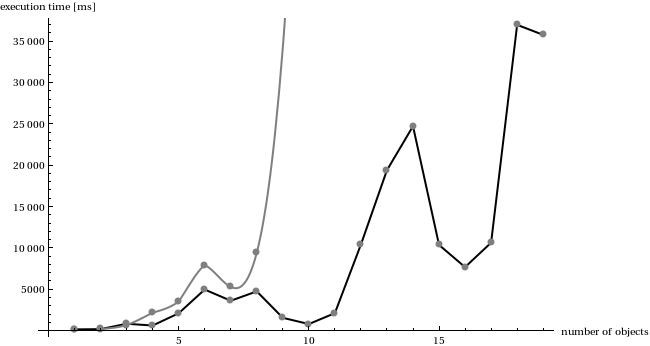
\includegraphics[scale=0.5]{figures/measurements_scalability}
\caption{Scalability results regarding the number of states or transitions}
\label{fig:measurements_scalability}
\end{figure}

The created model-based testing framework performs well, while generating test suites for medium sized models. Practically that means SUT with 5-10 states and 15-20 transitions are solvable by this tool. In this range the execution speed varies under 35 seconds, which is an acceptable speed.

Used input models were randomly generated test models, that's why the complexity of solving these problems does not perfectly follows the increase of the concerned testing objects. Besides that we can see a trend line, that the execution speed increases linear or polynomial at first, but later it will grow exponentially regarding the number of states or transitions.

Important to note that the number of states in the SUT model, affects the execution speed more, than the number of transitions, as possible states of the \texttt{System} (set of internal variables) are bound to the \texttt{State} objects in the Alloy model. So as the number of states increases, so does the possible value assignments for internal variables increases.

% section scalability (end)

% chapter measurements (end)